\documentclass{article}
\usepackage{tikz}

\begin{document}
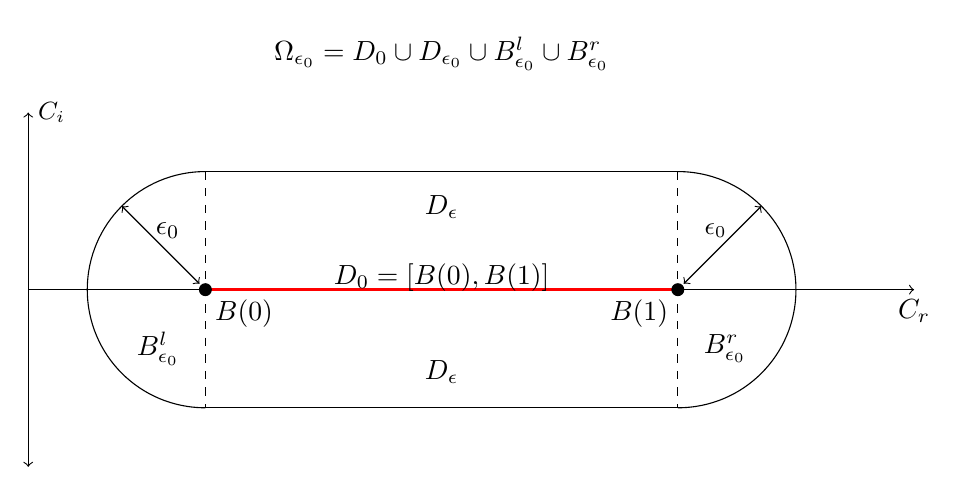
\begin{tikzpicture}[scale=1.5]
\draw[->] (0.5,0)--(8,0);
\node[below] at (8,0) {$C_r$};
\draw[<->] (0.5,-1.5)--(0.5,1.5);
\node[right] at (0.5,1.5) {\small $C_i$};
\draw (2,-1) to [out=180,in=270] (1,0) to [out=90,in=180] (2,1);
\draw[<->] (1.95,0.05)--(1.293,0.707);
\node at (1.68,0.5) {$\tiny \epsilon_0$};
\draw[<->] (6.05,0.05)--(6.707,0.707);
\node at (6.32,0.5) {\small $ \epsilon_0$};
\draw (2,1)--(6,1);
\draw (2,-1)--(6,-1);
\draw (6,1) to [out=0,in=90] (7,0) to [out=270,in=0] (6,-1);
\draw[dashed] (2,1)--(2,-1);
\draw[dashed] (6,1)--(6,-1);
\draw[draw=red, very thick] (2,0)--(6,0);
\node at (4,0.1) {$D_0=[B(0),B(1)]$};
\node at (4,0.7) {$D_{\epsilon}$};
\node at (4,-0.7) {$D_{\epsilon}$};
\draw[fill] (2,0) circle [radius=0.05];
\node[below right] at (2,0) {$\tiny B(0)$};
\draw[fill] (6,0) circle [radius=0.05];
\node[below left] at (6,0) {$\tiny B(1)$};
\node at (1.6,-0.5) {$B_{\epsilon_0}^l$};
\node at (6.4,-0.5) {$B_{\epsilon_0}^r$};
\node at (4,2) {$\Omega_{\epsilon_0}=D_0\cup D_{\epsilon_0} \cup 
B_{\epsilon_0}^l \cup B_{\epsilon_0}^r$};
\end{tikzpicture}
\end{document}
